\begingroup

\TPGrid{3}{36}
\textblockorigin{0mm}{0mm}
\setlength{\parindent}{0mm}
\setlength{\banderougewidth}{2\TPHorizModule}
\setlength{\banderougeheight}{\TPVertModule}
\setlength{\bandeorwidth}{\TPHorizModule}
\setlength{\bandeorheight}{\banderougeheight}
\setlength{\imageheight}{29\TPVertModule}
\setlength{\logoheight}{2.5\TPVertModule}
\setlength{\gapwidth}{0.75pt}
\addtolength{\bandeorwidth}{-\gapwidth}
\addtolength{\imageheight}{-\gapwidth}

\begin{frame}[plain]
  %% bandeau identitaire
  \begin{textblock*}{125mm}[0,1](0mm,30\TPVertModule)
    \textcolor{rouge}{\rule{\banderougewidth}{\banderougeheight}}% % bande rouge
    \rule{\gapwidth}{0pt}%                                         % filet
    \textcolor{or}{\rule{\bandeorwidth}{\bandeorheight}}           % bande or
  \end{textblock*}

  %% logo UL
  \begin{textblock*}{\TPHorizModule}(2\TPHorizModule,31\TPVertModule)
    \rule{\gapwidth}{0pt}%                                     % filet
    
\includegraphics[height=\logoheight,keepaspectratio=true]{ul_p}
  \end{textblock*}

  %% image de fond
  \begin{textblock*}{125mm}(0mm,0mm)
    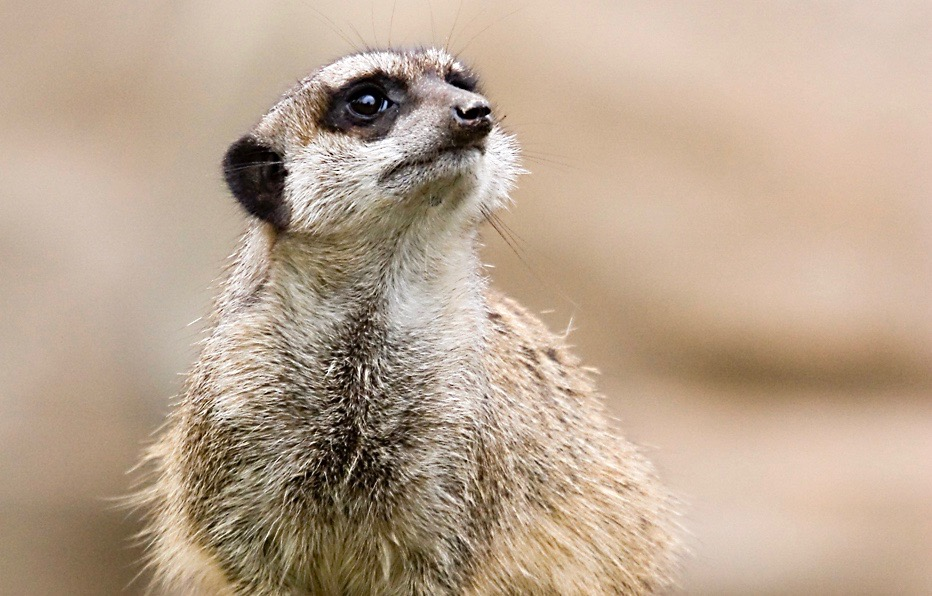
\includegraphics[height=\imageheight,keepaspectratio=true]{Suricata-diapos.jpg}
  \end{textblock*}

  %% trame (titre)
  \begin{textblock*}{2\TPHorizModule}(0mm,14\TPVertModule)
    \pgfsetfillopacity{0.5}
    \textcolor{white}{\rule{\linewidth}{10\TPVertModule}}
    \pgfsetfillopacity{1}
  \end{textblock*}

  %% titre
  \begin{textblock*}{1.6\TPHorizModule}(0.4\TPHorizModule,15.2\TPVertModule)
    \raggedright%
    \titles\bfseries
    \fontsize{20}{20}\selectfont
    Rédaction avec \\
    \rmfamily\mdseries
    \fontsize{22.5}{22.5}\selectfont
    \raisebox{5pt}{{\textbackslash}title}%
    \fontsize{40}{40}\selectfont%
    \{%
    \fontsize{35}{35}\selectfont%
    \LaTeX
    \fontsize{40}{40}\selectfont%
    \}
  \end{textblock*}

  %% trame (premiers pas)
  \begin{textblock*}{\TPHorizModule}(2\TPHorizModule,24\TPVertModule)
    \pgfsetfillopacity{0.5}
    \textcolor{white}{\rule{\linewidth}{2\TPVertModule}}
    \pgfsetfillopacity{1}
  \end{textblock*}

  %%
  \begin{textblock*}{0.8\TPHorizModule}(2.1\TPHorizModule,24.5\TPVertModule)
    \raggedright%
    \titles\bfseries
    \fontsize{11}{11}\selectfont
    Premiers pas
  \end{textblock*}
\end{frame}
\endgroup

%%% Local Variables:
%%% mode: latex
%%% TeX-engine: xetex
%%% TeX-master: "formation-latex-ul-diapos"
%%% End:
